\documentclass[
11pt, % The default document font size, options: 10pt, 11pt, 12pt
%codirector, % Uncomment to add a codirector to the title page
]{charter} 




% El títulos de la memoria, se usa en la carátula y se puede usar el cualquier lugar del documento con el comando \ttitle
\titulo{Extensión de plataforma de detección RFID Atheling} 

% Nombre del posgrado, se usa en la carátula y se puede usar el cualquier lugar del documento con el comando \degreename
\posgrado{Carrera de Especialización en Sistemas Embebidos} 
%\posgrado{Carrera de Especialización en Internet de las Cosas} 
%\posgrado{Carrera de Especialización en Intelegencia Artificial}
%\posgrado{Maestría en Sistemas Embebidos} 
%\posgrado{Maestría en Internet de las cosas}

% Tu nombre, se puede usar el cualquier lugar del documento con el comando \authorname
\autor{Mag. Ing. Andrade R. Edda G.} 

% El nombre del director y co-director, se puede usar el cualquier lugar del documento con el comando \supname y \cosupname y \pertesupname y \pertecosupname
\director{Esp. Ing. Abbate Santiago}
\pertenenciaDirector{EmTech} 
% FIXME:NO IMPLEMENTADO EL CODIRECTOR ni su pertenencia
\codirector{Falta Definir} % para que aparezca en la portada se debe descomentar la opción codirector en el documentclass
\pertenenciaCoDirector{Falta Definir}

% Nombre del cliente, quien va a aprobar los resultados del proyecto, se puede usar con el comando \clientename y \empclientename
\cliente{Mauro Koenig}
\empresaCliente{EmTech}

% Nombre y pertenencia de los jurados, se pueden usar el cualquier lugar del documento con el comando \jurunoname, \jurdosname y \jurtresname y \perteunoname, \pertedosname y \pertetresname.
\juradoUno{Nombre y Apellido (1)}
\pertenenciaJurUno{pertenencia (1)} 
\juradoDos{Nombre y Apellido (2)}
\pertenenciaJurDos{pertenencia (2)}
\juradoTres{Nombre y Apellido (3)}
\pertenenciaJurTres{pertenencia (3)}
 
\fechaINICIO{22 de agosto de 2023}		%Fecha de inicio de la cursada de GdP \fechaInicioName
\fechaFINALPlan{10 de octubre de 2023} 	%Fecha de final de cursada de GdP
\fechaFINALTrabajo{Agosto 2024}	%Fecha de defensa pública del trabajo final


\begin{document}

\maketitle
\thispagestyle{empty}
\pagebreak


\thispagestyle{empty}
{\setlength{\parskip}{0pt}
\tableofcontents{}
}
\pagebreak


\section*{Registros de cambios}
\label{sec:registro}


\begin{table}[ht]
\label{tab:registro}
\centering
\begin{tabularx}{\linewidth}{@{}|c|X|c|@{}}
\hline
\rowcolor[HTML]{C0C0C0} 
Revisión & \multicolumn{1}{c|}{\cellcolor[HTML]{C0C0C0}Detalles de los cambios realizados} & Fecha      \\ \hline
0      & Creación del documento                                 &\fechaInicioName \\ \hline
1      & Se completa hasta el punto 5 inclusive                 & 7 de septiembre de 2023 \\ \hline
2      & Se completa hasta el punto 9 inclusive y se agregan correcciones de la revisión 1  & 14 de septiembre de 2023 \\ \hline
3      & Se completa hasta el punto 9 inclusive y se agregan correcciones de la revisión 2  & 26 de septiembre de 2023 \\ \hline
%		  Se puede agregar algo más \newline
%		  En distintas líneas \newline
%		  Así                                                    & dd/mm/aaaa \\ \hline
%3      & Se completa hasta el punto 11 inclusive                & dd/mm/aaaa \\ \hline
%4      & Se completa el plan	                                 & dd/mm/aaaa \\ \hline
\end{tabularx}
\end{table}

\pagebreak



\section*{Acta de constitución del proyecto}
\label{sec:acta}

\begin{flushright}
Buenos Aires, \fechaInicioName
\end{flushright}

\vspace{2cm}

Por medio de la presente se acuerda con la \authorname\hspace{1px} que su Trabajo Final de la \degreename\hspace{1px} se titulará ``\ttitle'', consistirá esencialmente en la implementación de una etapa de autotuning para lograr el uso de la plataforma de detección RFID de Atheling con antenas de distinto alcance, y tendrá un presupuesto preliminar estimado de 785 h de trabajo, de las cuales 700 h son responsabilidad de la alumna, y 20228.5 USD, con fecha de inicio \fechaInicioName\hspace{1px} y fecha de presentación pública \fechaFinalName.

Se adjunta a esta acta la planificación inicial.

\vfill

% Esta parte se construye sola con la información que hayan cargado en el preámbulo del documento y no debe modificarla
\begin{table}[ht]
\centering
\begin{tabular}{ccc}
\begin{tabular}[c]{@{}c@{}}Dr. Ing. Ariel Lutenberg \\ Director posgrado FIUBA\end{tabular} & \hspace{2cm} & \begin{tabular}[c]{@{}c@{}}\clientename \\ \empclientename \end{tabular} \vspace{2.5cm} \\ 
\multicolumn{3}{c}{\begin{tabular}[c]{@{}c@{}} \supname \\ Director del Trabajo Final\end{tabular}} \vspace{2.5cm} \\
%\begin{tabular}[c]{@{}c@{}}\jurunoname \\ Jurado del Trabajo Final\end{tabular}     &  & \begin{tabular}[c]{@{}c@{}}\jurdosname\\ Jurado del Trabajo Final\end{tabular}  \vspace{2.5cm}  \\
%\multicolumn{3}{c}{\begin{tabular}[c]{@{}c@{}} \jurtresname\\ Jurado del Trabajo Final\end{tabular}} \vspace{.5cm}                                                                     
\end{tabular}
\end{table}




\section{1. Descripción técnica-conceptual del proyecto a realizar}
\label{sec:descripcion}

Con el crecimiento exponencial de la población mundial, la producción de alimentos cobró una relevancia fundamental en el mundo globalizado y moderno en el que vivimos. Es por ello que la automatización de los procesos productivos resulta de gran interés. 

Abastecer las grandes demandas de la industria cárnica requiere de un exhaustivo trabajo en zonas agrestes de gran extensión. Es por ello que la compañía EmTech desarrolló distintas plataformas marca Atheling, que se encargan de monitorear a los animales de forma automatizada y remota. Los sistemas de Atheling se encuentran instrumentados con múltiples sensores que permiten mantener un registro de los animales. Cada animal es identificado con un único ID (caravana electrónica HDX). Los datos recolectados por las antenas de Atheling se transmiten y procesan de modo tal que el productor tiene todas las variables relevantes disponibles al alcance de dispositivos de uso cotidiano, como un celular. Esto permite la toma de decisiones en tiempo real, fundamentadas en datos concretos, con la finalidad de optimizar la producción.  

En el marco de la aplicación antes mencionada, la compañía EmTech requiere extender la actual plataforma de detección de animales, para lograr obtener una lectura confiable de las caravanas electrónicas portadas por éstos desde distintas antenas y en distintas condiciones ambientales, rediseñándola para incluir un nuevo microprocesador de ultra bajo consumo. El objetivo del proyecto es portar el código al nuevo microprocesador e implementar una etapa de autosintonización que maximice la señal recibida desde las antenas de Atheling de corto y largo alcance. 

El proyecto presentado en este documento es parte del programa de vinculación con empresas y tiene como objetivo implementar la extensión de la plataforma de detección RFID introducida anteriormente, la cual actualmente se encuentra en uso. Para ello es necesario calcular y simular la etapa de autosintonización con ambas antenas (largo y corto alcance), actualizar el diseño del circuito impreso, generar los archivos de fabricación, portar y actualizar el firmware para que el nuevo microprocesador realice la sintonización con ambas antenas. Por último, se requiere realizar pruebas de validación y un informe de sus resultados. El proyecto será llevado a cabo por la autora de este documento en conjunto con colaboradores de la compañía EmTech.

La etapa de autosintonización con las antenas se realiza por medio de un banco de capacitores con llaves, cuya conmutación es comandada por el microcontrolador embebido en la plataforma. Dicho microcontrolador detecta de forma automática la combinación óptima de capacitores para lograr comunicarse con cada antena. En la Figura 1 se muestra un diagrama de bloques de la solución. El color marrón representa la plataforma como es actualmente, mientras que el color azul muestra la propuesta de extensión.




\begin{figure}[htpb]
\centering 
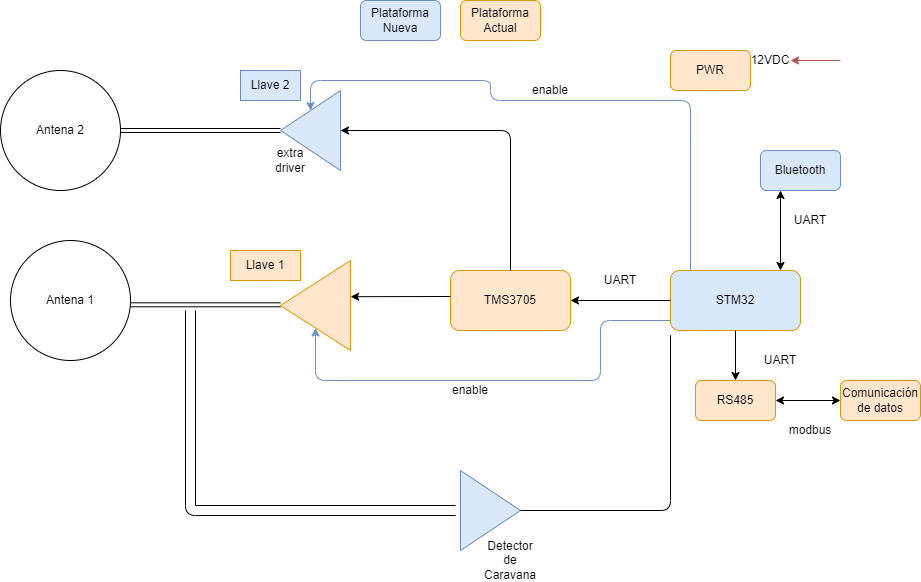
\includegraphics[width=1\textwidth]{./Figuras/Diagrama-de-bloques.png}
\caption{Diagrama en bloques del sistema}
\label{fig:diagBloques}
\end{figure}

\vspace{25px}


\section{2. Identificación y análisis de los interesados}
\label{sec:interesados}



\begin{table}[ht]
%\caption{Identificación de los interesados}
%\label{tab:interesados}
\begin{tabularx}{\linewidth}{@{}|l|X|X|l|@{}}
\hline
\rowcolor[HTML]{C0C0C0} 
Rol           & Apellido y Nombre & Organización 	& Puesto 	\\ \hline
Cliente       & \clientename      &\empclientename	&-       	\\ \hline
Responsable   & \authorname       & FIUBA        	& Alumna 	\\ \hline
Colaboradores & Pedranti Fernando & Atheling      	& Socio    	\\ \hline
Orientador    & \supname	      & \pertesupname 	& Director Trabajo final \\ \hline
%Equipo        & Falta definir
%				          &       -       	& -       	\\ \hline

\end{tabularx}
\end{table}



\section{3. Propósito del proyecto}
\label{sec:proposito}

El propósito de este proyecto es extender el uso de la plataforma de Atheling de detección de animales portadores de caravanas electrónicas para ser utilizada con diferentes antenas, implementado con un microcontrolador de ultra bajo consumo.


\section{4. Alcance del proyecto}
\label{sec:alcance}

El alcance de este proyecto comprende las siguientes actividades:
\begin{itemize}
	\item Simular y calcular de la etapa de autosintonización.
	\item Rediseñar y fabricar un prototipo.
	\item Adaptar el firmware al nuevo microcontrolador de ultra bajo consumo.
	\item Actualizar el firmware para que el microcontrolador realice de forma automática la sintonización con cada antena.
	\item Planificar y realizar las pruebas de validación del prototipo.
	\item Elaborar un informe de validación del circuito actualizado.
\end{itemize}
Como se especifica en la lista anterior, este proyecto no pretende entregar un equipo integrado en funcionamiento listo para su comercialización sino un prototipo. Cabe mencionar que todas las actividades enlistadas no son responsabilidad exclusiva de la autora de este documento, sino que serán realizadas en conjunto con colaboradores y miembros del equipo de la compañía EmTech-Atheling. 

\section{5. Supuestos del proyecto}
\label{sec:supuestos}

Para lograr el éxito de este proyecto se realizan las siguientes suposiciones:

\begin{itemize}
	\item EmTech realizó una primera aproximación de cálculo para corroborar que el hardware actual sea compatible con la aplicación requerida.
	\item EmTech define los requerimientos detallados y el criterio de aceptabilidad de los entregables.
	\item EmTech pone a disposición toda la información necesaria, con el nivel de detalle adecuado.
	\item La alumna y todos las personas involucradas acuerdan la dinámica laboral, realizando un desgloce de tareas, asignándolas a quien corresponda. 
	\item EmTech asigna los recursos humanos competentes para llevar a cabo el rediseño y fabricación del prototipo en un plazo de tiempo acotado (falta acordar dicho plazo con la compañía).
	\item EmTech financia la fabricación del prototipo.
	\item EmTech pone a disposición el hardware necesario para realizar las pruebas de validación del prototipo.
	\item El Director de Proyecto asignado tiene las competencias y la disponibilidad de tiempo necesarios para guiar a la alumna en las tareas específicas de este proyecto. 
	\item La alumna dispone de tiempo para dedicar al proyecto de no menos de 10 h semanales hasta su culminación.
	
\end{itemize}


\section{6. Requerimientos}
\label{sec:requerimientos}


\begin{enumerate}
	\item Requerimientos generales de funcionalidad\\
	El sistema debe:
		\begin{enumerate}
			\item  Leer etiquetas RFID HDX bajo el estándar ISO 11785.
			\item  Sintonizar automáticamente  la etapa de radiofrecuencia para lectura de las etiquetas.
			\item  Leer las etiquetas hasta una distancia máxima de 60 cm.
			\item  Indicar mediante un estímulo sonoro la correcta lectura de una etiqueta.
			\item  Implementar una comunicación MODBUS vía RS485 para la recepción de comandos de control y lectura de datos.
			\item  Comandar una salida a relé normal abierta, vía la recepción de un comando a través de la interfaz MODBUS.
			\item  Contar con la posibilidad de utilizar una o dos antenas, configurable vía selectores en el PCB.
			\item Contar con un módulo Bluetooth para lectura en sitio de las etiquetas detectadas. 

		\end{enumerate}
	\item Requerimientos de desarrollo del prototipo 
		\begin{enumerate}
			\item El desarrollo del prototipo debe basarse en la plataforma de lectura Atheling RFID V1.
			\item La decodificación de las etiquetas  debe implementarse con base en el circuito integrado TMS3705.
			\item El control y procesamiento de datos del sistema debe basarse en un microcontrolador STM32L152CBT6.
			\item La plataforma debe contar con una interfaz para su programación mediante un programador externo. El programador y depurador USB ST-Link debe tenerse en cuenta como sugerencia.
			\item Se deben mantener las dimensiones 2D y fijaciones de la plataforma Atheling RFID V1.
			\item Se deben implementar cambios en el circuito de potencia y en el tamaño de los agujeros.
			
		\end{enumerate}
	\item Requerimientos de firmware
	\begin{enumerate}
			\item Portar y/o rehacer el firmware actual para que funcione en el nuevo microcontrolador. 
			\item Desarrollar el código para autosintonización.
			\item Desarrollar drivers para las interfaces de programación, Módulo BLE, RS485, otros periféricos como alarmas sonoras, llaves, y los circuitos integrados necesarios para cumplir con los requerimientos funcionales de este documento.
			\end{enumerate}
	\item Requerimientos de control de cambios
	\begin{enumerate}
			\item Se debe mantener actualizadas las versiones de código mediante el uso del repositorio de EmTech.
			\end{enumerate}
	
	\item Requerimientos documentales
	\begin{enumerate}
			\item Se debe realizar la documentación de desarrollo del código de acuerdo a los lineamientos de documentación de EmTech. 
			\item Se debe realizar la documentación de desarrollo del código de acuerdo a los lineamientos de documentación de EmTech.
			\item Se debe entregar el informe de avance y la memoria técnica de este proyecto, de acuerdo con los requerimientos de esta casa de altos estudios.
			\end{enumerate}
			\item Requerimientos de validación y pruebas
	\begin{enumerate}
			\item Se deberá validar el funcionamiento del prototipo mediante pruebas de laboratorio que simulen escenarios de uso de la plataforma.
			\end{enumerate}
\end{enumerate}



\section{7. Historias de usuarios (\textit{Product backlog})}
\label{sec:backlog}

A continuación se enumeran las historias de usuarios identificadas. Para poder medir el tama˜no de cada historia se ha realizado una ponderación numérica con base en la serie de Fibonacci 0,
1, 2, 3, 5, 8, 13, 21, 34, 55, .... Los criterios y las ponderaciones consideradas son las siguientes:
\begin{enumerate}
\item Dificultad del trabajo
      \begin{itemize}
      \item Bajo = 1
      \item Medio = 5
      \item Alto = 13
      \end{itemize}
\item Complejidad del trabajo
      \begin{itemize}
      \item Bajo = 2
      \item Medio = 5
      \item Alto = 13
      \end{itemize}
\item Riesgo del trabajo
      \begin{itemize}
      \item Bajo = 1
      \item Medio = 3
      \item Alto = 8
      \end{itemize}
\end{enumerate}
Luego, cada historia de usuario obtiene un puntaje (Story Points) que resulta de aproximar la suma de su dificultad, su complejidad y su riesgo al número más cercano de la serie de Fibonacci.

\subsection{Historia de Cuidador de Animales}

``Como cuidador de animales quiero poder identificar a cada animal, para contarlos y evitar pérdidas''
\begin{enumerate}
      \item Dificultad = 5
      \item Complejidad = 2
      \item Riesgo = 3
\end{enumerate}
 Total: \textbf{Storypints = 8}

\subsection{Historia del Zootécnico} 
``Como zootécnico quiero balancear la alimentación de los animales para que el engorde sea parejo, para ello necesito identificar cada animal y su historial de peso''
\begin{enumerate}
      \item Dificultad = 13
      \item Complejidad = 5
      \item Riesgo = 3
\end{enumerate}
 Total: \textbf{Storypints = 21 }
 
\subsection{Historia del dueño del campo}
``Como dueño del campo quiero tener la información al alcance de la mano para dar seguimiento y tomar decisiones estratégicas sobre mis animales.''
\begin{enumerate}
      \item Dificultad = 13 
      \item Complejidad = 13
      \item Riesgo = 3
\end{enumerate}
 Total: \textbf{Storypints = 34 }

\subsection{Historia del encargado de soporte técnico} 
``Como encargado de soporte técnico quiero evitar dificultades en la instalación de los nodos, por lo que necesito que el lector tenga una buena relación señal/ruido, para evitar lecturas espúrias.''
\begin{enumerate}
      \item Dificultad = 5
      \item Complejidad = 13
      \item Riesgo = 3
\end{enumerate}
 Total: \textbf{Storypints = 21 }
 
\subsection{Historia del impulsor del proyecto} 
``Como impulsor del proyecto quiero ampliar la plataforma para lograr robustez ante el ruido electromagnético para poder usar nuestros equipos en zonas más urbanizadas y en distintas condiciones de montaje, por ejemplo, sobre estructuras metálicas que afecten las características de las antenas.''
\begin{enumerate}
      \item Dificultad = 5
      \item Complejidad = 13
      \item Riesgo = 3
\end{enumerate}
 Total: \textbf{Storypints = 21 }
 


\section{8. Entregables principales del proyecto}
\label{sec:entregables}

Los entregables del proyecto son:

\begin{itemize}
	\item Documento de ingeniería de la aplicación del circuito, análisis de lo que se agrega, fundamentos y líneas para hacer el esquemático + PCB.
    \item Documentos de fabricación del PCB (Gerbers + archivo de fabricación + P and P).
    \item Esquemáticos del PCB + BOM.
	\item Código fuente del firmware.
	\item Documentación del código.
	\item Informe de cierre del proyecto.
	\item Informe de avance.
	\item Memoria técnica.

\end{itemize}


\section{9. Desglose del trabajo en tareas: 785 h totales, a cargo de la alumna 700 h } 
\label{sec:wbs}

\begin{enumerate}
\item Planificación del proyecto: 78 h
	\begin{enumerate}
	\item Definir el alcance del proyecto: 10 h
	\item Acordar metodologías de trabajo, gestión de la información, medios de comunicación: 20 h
	\item Gestionar los recursos para asegurar la disponibilidad en el momento de realización de las pruebas: 40 h
	\item Confeccionar el Plan de Trabajo: 48 h
	\end{enumerate}

\item Simulación y cálculo de la etapa de autosintonización: 45 h
	\begin{enumerate}
	\item Investigar el estado del arte: 40 h
	\item Calcular el circuito: 20 h
	\item Simular el comportamiento del circuito: 20 h 
	\end{enumerate}
	
\item Diseño del prototipo: 141 h
	\begin{enumerate}
	\item Selecionar los componentes: 20 h
	\item Calcular los circuitos: 10 h
	\item Diseñar los circuitos esquemáticos: 20 h
	\item Confeccionar las memorias de cálculo: 10 h
	\item Confeccionar el Bill Of Materials (BOM): 5 h
	\item Confeccionar los esquemáticos entregables: 20 h
	\item Diseñar el PCB: 40 h
	\item Confeccionar los documentos de fabricación (gerbers, Pick and Place, etc.): 10 h
	\item Modelar CAD 3D del PCB: 5 h
	\item Verificar la compatibilidad mecánica/espacial del PCB dentro del gabinete: 1 h
	\end{enumerate}
	
\item Fabricación del prototipo: 120 h
	\begin{enumerate}
	\item Buscar proveedores y solicitar cotizaciones: 20 h (a cargo de EmTech)
	\item Rediseñar el PCB en función de la retroalimentación con el/los fabricantes: 10 h 
	\item Dar seguimiento a la fabricación: 10 h
	\item Fabricar el PCB y montar componentes: 40 h (a cargo de EmTech)
	\item Integrar el sistema embebido al gabinete, con sus fijaciones, fuente de alimentación, etc.: 40 h
    \end{enumerate}
    
\item Desarrollo de Firmware: 172 h
	\begin{enumerate}
	\item Estudiar el código actual: 10 h
	\item Evaluar si recodificar completamente el código o portar: 2 h
	\item Portar/recodificar las funcionalidades actuales para que funcionen en el nuevo microcontrolador: 40 h
	\item Desarrollar drivers para las interfaces de comunicación, programación y periféricos como alarma sonora: 80 h
	\item Desarrollar el código de autosintonización: 40 h
	\end{enumerate}

\item Prueba del firmware: 45 h
    \begin{enumerate}
    \item Montar periféricos de prueba para verificación de funcionamiento del firmware: 5 h
    \item Analizar y depurar el código: 40 h
    \end{enumerate}

\item Diseño de pruebas de validación: 25 h
    \begin{enumerate}
    \item Definir criterios de aceptación del comportamiento de la plataforma: 20 h (a cargo de EmTech)
    \item Definir el alcance de las pruebas a realizarse: 2 h (a cargo de EmTech)
    \item Definir los recursos necesarios (espacio, instrumentación, personal, etc): 5 h (a cargo de EmTech)
    
    \end{enumerate}
    
\item Pruebas de validación: 70 h
    \begin{enumerate}
    \item Realizar pruebas de validación: 60 h
    \item Documentar pruebas de validación: 10 h
    \end{enumerate}
    
\item Presentación final del proyecto: 89 h
    \begin{enumerate}
    \item Confeccionar el informe de avance: 30 h
    \item Confeccionar la memoria técnica: 30 h
    \item Confeccionar la presentación pública: 20 h
    \item Practicar la presentación en conjunto con el director: 5 h
    \end{enumerate}

  
\end{enumerate}


\section{10. Diagrama de Activity On Node}
\label{sec:AoN}

\begin{figure}
	\centering
	
	\begin{tikzpicture}[node distance=2.5cm]
	
	\tikzstyle{block} = [rectangle, draw, fill=cyan!40, 
	text width=10em, text centered, rounded corners, minimum height=3em]
	\tikzstyle{criticalblock} = [rectangle, draw, fill=magenta!40, 
	text width=10em, text centered, rounded corners, minimum height=3em]
	\tikzstyle{line} = [draw, -latex']
	
	\node [block] (init) {Inicio 22/08/2023};
	\node [block, below of=init]              	    (1) {1.Planificación del Proyecto:78 h };
	\node [block, below of=1]                  	    (2) {2.Simulación y Cálculo de la etapa de autosintonización: 45 h};
	\node [block, below of=2]	                    (3) {3.Diseño del prototipo: 141 h};
	\node [criticalblock, below of=3, left of=3, node distance=4cm]                       (4) {4.Fabricación del prototipo: 120 h};
	\node [block, below of=3, right of=3, node distance=4cm]    (5) {5.Desarrollo de Firmware: 172 h};
	\node [block, below of=5]                  	    (6) {6.Prueba de Firmware: 45 h};
	\node [block, below of=4]                    	(7) {7.Diseño de pruebas de validación: 27 h};
	\node [criticalblock, below of=7, node distance=2.5cm,right of=7, node distance=4cm] 				    	(8) {8.Pruebas de Validación: 70 h};
	\node [block, below of=8] 					    (9) {9.Presentación Final del proyecto: 89 h };
	\node [criticalblock, below of=9]                       (10){Defensa Pública 01/08/2024};

\node [rectangle, draw, fill=magenta!40, 
	text width=6em, text centered, rounded corners, minimum height=1em, left of=1, node distance=6cm] (leyenda2) {actividad crítica};	
	
	\path [line] (init) -> 	(1);
	\path [line] (1) 	-> 	(2);
	\path [line] (2) 	-> 	(3);
	\path [line] (3) 	|-  (4);
	\path [line] (3) 	|- 	(5);
	\path [line] (4) 	-> 	(7);
	\path [line] (5) 	-- 	(6);
	\path [line] (6) 	|- 	(8);
	\path [line] (7) 	|- 	(8);
	\path [line] (8) 	-- 	(9);
	\path [line] (9) 	-- 	(10);
	
	
	\end{tikzpicture}
	\caption{Diagrama AoN}
\end{figure}

\section{11. Diagrama de Gantt}
\label{sec:gantt}
En las siguientes páginas se muestra el Diagrama de Gantt de acuerdo al WBS descripto en la sección 9.

\begin{landscape}
%\rotatebox{90}{%
\begin{ganttchart}[
	hgrid,
vgrid,
	x unit=0.15cm,
	y unit chart=1cm,
time slot format=isodate,
time slot unit=day,
bar/.append style={fill=cyan!30},
group/.append style={fill=magenta!50},
bar/.append style={fill=cyan!30, bar label node/.append style={above=3pt}},
%include title in canvas=false,
%inline,
milestone inline label node/.append style={left=5mm}
%link/.style={->, thick}
%link label font=\small\bfseries\color{purple}
link/.style={|-to, line width=0.5pt, magenta},
    bar inline label node/.style={
	anchor=east,
	xshift=+4.5cm,
	yshift=0.4cm,
}]{2023-08-22}{2023-12-16}
	
%{\small
	\gantttitlecalendar{year, month} \\
	
	\ganttgroup{1 Planificación del Proyecto}{2023-08-22}{2023-10-10} \\
	\ganttbar[name=11]{1.1 Definir el alcance del proyecto}{2023-08-22}{2023-08-30} \\
	\ganttbar[name=12]{1.2 Acordar metodologías de trabajo}{2023-09-01}{2023-09-10} \\
	\ganttbar[name=13]{1.3 Gestionar los recursos}{2023-08-22}{2023-10-10} \\
	\ganttbar[name=14]{1.4 Confeccionar el Plan de Trabajo}{2023-08-22}{2023-10-10} \\
	
	\ganttmilestone{Presentación del Plan de Trabajo}{2023-10-10}\\ 	
	
	\ganttgroup{2 Simulación y cálculo}{2023-10-16}{2023-12-16} \\
	\ganttbar[name=21]{2.1 Investigar el estado del arte}{2023-10-16}{2023-11-15} \\
	\ganttbar[name=22]{2.2 Calcular el circuito}{2023-11-18}{2023-12-02} \\
	\ganttbar[name=23]{2.3 Simular el comportamiento del circuito}{2023-12-02}{2023-12-16} \\
	
	\ganttlink[]{21}{22}
	\ganttlink[]{22}{23}

\end{ganttchart}
%}
%\end{landscape}


%\begin{landscape}
%\rotatebox{90}{%
\newpage
\begin{ganttchart}[
	hgrid,
vgrid,
	x unit=0.146cm,
	y unit chart=0.85cm,
time slot format=isodate,
time slot unit=day,
bar/.append style={fill=cyan!30},
group/.append style={fill=magenta!50},
bar/.append style={fill=cyan!30, bar label node/.append style={above=3pt}},
%include title in canvas=false,
%inline,
milestone inline label node/.append style={left=5mm}
%link/.style={->, thick}
%link label font=\small\bfseries\color{purple}
link/.style={|-to, line width=0.5pt, magenta},
    bar inline label node/.style={
	anchor=east,
	xshift=+4.5cm,
	yshift=0.4cm,
}]
{2023-12-16}{2024-04-10}
	
	\gantttitlecalendar{year, month} \\
	
	\ganttgroup{3 Diseño del prototipo}{2023-12-18}{2024-02-09}\\
	\ganttbar[name=31]{3.1 Seleccionar los componentes}{2023-12-18}{2023-12-20} \\
	\ganttbar[name=32]{3.2 Calcular circuitos}{2023-12-20}{2023-12-21} \\
	\ganttbar[name=33]{3.3 Diseñar esquemáticos}{2024-01-02}{2024-01-04} \\
	\ganttbar[name=34]{3.4 Confeccionar memorias}{2024-01-04}{2024-01-05} \\
	\ganttbar[name=35]{3.5 Confeccionar BOM}{2024-01-05}{2024-01-06} \\
	\ganttbar[name=36]{3.6 Confeccionar los esquemáticos entregables}{2024-01-08}{2024-01-10} \\
	\ganttbar[name=37]{3.7 Diseñar PCB}{2024-01-10}{2024-02-07} \\
	\ganttbar[name=38]{3.8 Confeccionar documentos de fabricación}{2024-02-07}{2024-02-08}\\
	\ganttbar[name=39]{3.9 Modelar 3D del PCB}{2024-02-08}{2024-02-09} \\
	\ganttbar[name=310]{3.10 Verificar la compatibilidad mecánica}{2024-02-09}{2024-02-09} \\
	
	
	\ganttgroup{4 Fabricación del prototipo}{2024-02-09}{2024-04-07} \\
	\ganttbar[name=41]{4.1 Gestión de compras}{2024-02-09}{2024-02-15} \\
	\ganttbar[name=42]{4.2 Rediseñar el PCB}{2024-02-09}{2024-02-15} \\
	\ganttbar[name=43]{4.3 Dar seguimiento a la fabricación}{2024-02-15}{2024-03-07} \\
    \ganttbar[name=44]{4.4 Montaje y puesta en marcha inicial}{2024-03-07}{2024-04-07} \\
	\ganttbar[name=45]{4.5 Integrar el sistema embebido}{2024-03-07}{2024-04-07} \\
	\ganttmilestone[name=46]{Prototipo Integrado con HW funcionando}{2024-04-07}

\ganttlink[]{32}{31}
\ganttlink[]{32}{33}
\ganttlink[]{32}{34}
\ganttlink[]{35}{37}	
\ganttlink[]{37}{38}
\ganttlink[]{39}{310}

\ganttlink[]{43}{42}
\ganttlink[]{43}{41}
\ganttlink[]{45}{43}
\ganttlink[]{44}{43}
\ganttlink[]{46}{44}
\ganttlink[]{46}{45}

\end{ganttchart}
%}
%\end{landscape}


%\begin{landscape}
%\rotatebox{90}{%
\newpage
\begin{ganttchart}[
	hgrid,
vgrid,
	x unit=0.263cm,
	y unit chart=0.85cm,
time slot format=isodate,
time slot unit=day,
bar/.append style={fill=cyan!30},
group/.append style={fill=magenta!50},
bar/.append style={fill=cyan!30, bar label node/.append style={above=3pt}},
%include title in canvas=false,
%inline,
milestone inline label node/.append style={left=5mm}
%link/.style={->, thick}
%link label font=\small\bfseries\color{purple}
link/.style={|-to, line width=0.5pt, magenta},
    bar inline label node/.style={
	anchor=east,
	xshift=+4.5cm,
	yshift=0.4cm,
}
]{2024-04-07}{2024-06-7}

	
	\gantttitlecalendar{year, month} \\
	
	\ganttgroup{5 Desarrollo de Firmware}{2024-04-07}{2024-05-28} \\
	\ganttbar[name=51]{5.1 Estudiar el código actual}{2024-04-07}{2024-04-08} \\
	\ganttbar[name=52]{5.2 Evaluar si recodificar o portar}{2024-04-08}{2024-04-11} \\
	\ganttbar[name=53]{5.3 Portar/recodificar las funcionalidades actuales}{2024-04-08}{2024-04-30} \\
	\ganttbar[name=54]{5.4 Desarrollar drivers}{2024-04-30}{2024-5-10}\\
	\ganttbar[name=55]{5.5 Desarrollar código de autosintonización}{2024-05-10}{2024-05-27} \\
	\ganttmilestone[name=56]{Presentación al cliente del Código}{2024-05-28} \\
	
	\ganttgroup{6 Prueba del firmware}{2024-04-07}{2024-06-07}\\
	\ganttbar[name=61]{6.1 Montar periféricos de prueba 
}{2024-04-07}{2024-04-30} \\
	\ganttbar[name=62]{6.2 Prueba de FW y corrección de bugs}{2024-05-28}{2024-06-07} \\
	\ganttgroup{7 Diseño de pruebas de validación}{2024-05-28}{2024-06-07} \\
	\ganttbar[name=71]{7.1 Definir criterios de aceptación}{2024-05-28}{2024-06-02} \\
	\ganttbar[name=72]{7.2 Definir el alcance de las pruebas}{2024-06-02}{2024-06-03} \\
	\ganttbar[name=73]{7.3 Definir los recursos necesarios}{2024-06-03}{2024-06-03}  \\

	\ganttlink[]{51}{52}
	\ganttlink[]{52}{53}
	\ganttlink[]{52}{54}
	\ganttlink[]{53}{55}
	
	\ganttlink[]{56}{55}
	\ganttlink[]{53}{54}	
	
	
	\ganttlink[]{72}{71}
	\ganttlink[]{73}{72}
	
	\ganttlink[]{61}{62}

	


\end{ganttchart}
%\end{landscape}
%}


%\rotatebox{90}{%
\newpage
%\begin{landscape}
\begin{ganttchart}[
	hgrid,
	vgrid,
	x unit=0.31cm,
	y unit chart=1cm,
	time slot format=isodate,
	time slot unit=day,
	bar/.append style={fill=cyan!30},
	group/.append style={fill=magenta!50},
	link/.style={->, thick}
	]{2024-06-08} {2024-08-03}
	
	\gantttitlecalendar{year, month} \\
	
	\ganttgroup{8 Pruebas de validación}{2024-06-08}{2024-07-08} \\
	\ganttbar[name=81]{8.1 Realizar pruebas de validación}{2024-06-08}{2024-07-07} \\
	\ganttmilestone{Culminación de las pruebas de validación}{2024-07-07} \\
	\ganttbar[name=82]{8.2 Documentar pruebas de validación}{2024-07-07}{2024-07-08}\\
	
	
	
	
	\ganttgroup{9 Presentación final del proyecto}{2024-06-08} {2024-08-03} \\
	\ganttbar[name=91]{9.1 Confeccionar el informe de avance}{2024-07-07}{2024-07-15} \\
	\ganttmilestone{Presentación del Avance del Proyecto}{2024-07-20} \\
	\ganttbar[name=92]{9.2 Confeccionar la memoria del proyecto}{2024-06-08} {2024-08-03} \\
	\ganttbar[name=93]{9.3 Confeccionar la presentación pública}{2024-07-21}{2024-07-28} \\
	\ganttbar[name=94]{9.4 Practicar presentación}{2024-07-28}{2024-07-29} \\
	\ganttmilestone{Defensa Pública del Proyecto}{2024-08-01}

%	\ganttlink[]{53}{55}
%	\ganttlink[]{53}{55}
%	\ganttlink[]{53}{55}
%	\ganttlink[]{53}{55}
%	\ganttlink[]{53}{55}

	
	
\end{ganttchart}
\end{landscape}
%}
	

\section{12. Presupuesto detallado del proyecto}
\label{sec:presupuesto}

\begin{table}[htpb]
\centering
\begin{tabularx}{\linewidth}{@{}|X|c|r|r|@{}}
\hline
\rowcolor[HTML]{C0C0C0} 
\multicolumn{4}{|c|}{\cellcolor[HTML]{C0C0C0}COSTOS DIRECTOS} \\ \hline
\rowcolor[HTML]{C0C0C0} 
Descripción &
  \multicolumn{1}{c|}{\cellcolor[HTML]{C0C0C0}Cantidad} &
  \multicolumn{1}{c|}{\cellcolor[HTML]{C0C0C0}Valor unitario} &
  \multicolumn{1}{c|}{\cellcolor[HTML]{C0C0C0}Valor total} \\ \hline
Horas de Ingeniería&
  \multicolumn{1}{c|}{837 h} &
  \multicolumn{1}{c|}{20 USD/h} &
  \multicolumn{1}{c|}{16740 USD} \\ \hline
Prototipo: Fabricación y Montaje&
  \multicolumn{1}{c|}{3 unidades} &
  \multicolumn{1}{c|}{250 USD/unidad} &
  \multicolumn{1}{c|}{750 USD} \\ \hline
\multicolumn{1}{|l|}{Componentes para validación y desarrollo} &1
   &100 USD
   &100 USD
   \\ \hline

\multicolumn{3}{|c|}{SUBTOTAL} &
  \multicolumn{1}{c|}{17590 USD} \\ \hline
\rowcolor[HTML]{C0C0C0} 
\multicolumn{4}{|c|}{\cellcolor[HTML]{C0C0C0}COSTOS INDIRECTOS} \\ \hline
\rowcolor[HTML]{C0C0C0} 
Descripción &
  \multicolumn{1}{c|}{\cellcolor[HTML]{C0C0C0}Cantidad} &
  \multicolumn{1}{c|}{\cellcolor[HTML]{C0C0C0}Valor unitario} &
  \multicolumn{1}{c|}{\cellcolor[HTML]{C0C0C0}Valor total} \\ \hline
\multicolumn{1}{|l|}{Costos indirectos 0,15* costos directos} &1
&2638 USD
   &2638 USD
   \\ \hline
\multicolumn{3}{|c|}{SUBTOTAL} &
  \multicolumn{1}{c|}{2638 USD} \\ \hline
\rowcolor[HTML]{C0C0C0}
\multicolumn{3}{|c|}{TOTAL} & 20228.5 USD
   \\ \hline
\end{tabularx}%
\end{table}

Como los valores son expresados en dólares estadounidenses, para estimar el valor en pesos argentinos, se toma la cotización de divisas oficial del BNA venta del día 27/09/2023: 350 ARS/USD. De esta manera el total del presupuesto del proyecto es 7.079.975 ARS.

\section{13. Gestión de riesgos}
\label{sec:riesgos}


Riesgo 1: Errores de diseño del PCB que derivan en imposibilidad de fabricación y/o montaje de componentes
\begin{itemize}
	\item Severidad (S): 8. Se asigna este valor de severidad ya que de ocurrir este evento el proyecto no puede continuar y de debe empezar nuevamente con el diseño para corregir estos errores
	\item Ocurrencia (O): 3. Se asigna este valor ya que los archivos de fabricación serán revisados por profesionales experimentados en la fabricación de este tipo de sistemas embebidos.
\end{itemize}

 
Riesgo 2: Falta de disponibilidad de componentes electrónicos
\begin{itemize}
	\item Severidad (S): 10. Se asigna este valor de severidad ya que, por ejemplo, si no se lograse conseguir el microprocesador hay que rehacer todo el proyecto, incluyendo el diseño del PCB, el firmware, drivers, etc.\\
	Justificar el motivo por el cual se asigna determinado número de severidad (S).
	\item Probabilidad de ocurrencia (O): 6. Se asigna este valor de probabilidad de ocurrencia debido a que en el pasado ya ocurrió una escacez de componentes de estas características y en el contexto macro-económico del país existe demasiada incertidumbre y dificultades para la importación de este tipo de componentes.\\
	
\end{itemize}   

Riesgo 3: Fallas durante el montaje de componentes electrónicos
\begin{itemize}
	\item Severidad (S): 9. Se asigna este valor ya que este tipo de fallas deriva en gastos adicionales de reparación o bien pueden dejar inutilizables componentes y/o circuitos impresos, dejando como consecuencia una gran pérdida tanto material como de tiempo.
	\item Ocurrencia (O): 7. Se asigna este valor ya que el proceso de montaje de los componentes se realiza en un laboratorio con un proceso artesanal no automatizado.
\end{itemize}

Riesgo 4: Fallas durante las pruebas de validación que derivan en el descarte del sistema embebido
\begin{itemize}
	\item Severidad (S): 10. Se asigna este valor ya que la ocurrencia de esta falla deriva en el descarte del sistema embebido con su consecuente pérdida económica.
	\item Ocurrencia (O): 3. Se asigna este valor de probabilidad baja ya que la alumna cuenta con amplia experiencia en laboratorios con el uso de dispositivos electrónicos de alta complejidad y en la integración de sistemas embebidos a sistemas fisicos.
\end{itemize}

Riesgo 5: Demoras excesivas en la fabricación y/o entrega del prototipo
\begin{itemize}
	\item Severidad (S): 7. Se asigna este valor ya que la ocurrencia de este evento retrasaría al proyecto.
	\item Ocurrencia (O): 5. Se asigna este valor ya que es habitual experimentar demoras en envíos internacionales.
\end{itemize}

Riesgo 6: El firmware es poco eficiente y tiene fallas aleatorias
\begin{itemize}
	\item Severidad (S): 5. Se asigna este valor ya que el sistema de detección de animales no es crítico, es decir no pone en riesgo la integridad física de ningún ser vivo ni la integridad de los circuitos.
	\item Ocurrencia (O): 3. Se asigna este valor ya que la alumna utilizará los lineamientos de desarrollo de software de EmTech y las buenas prácticas de programación aprendidas en la CESE. 
\end{itemize}

Riesgo 7: EmTech evalúa y decide no continuar con el proyecto
\begin{itemize}
	\item Severidad (S): 10. Se asigna este valor ya que implicaría el cierre del proyecto. 
	\item Ocurrencia (O): 1. Se asigna este valor ya que según lo pactado con EmTech el proyecto cuenta con el impulso necesario para llevarse a cabo en el tiempo estipulado en el presente documento. 
\end{itemize}

\newpage
En la siguiente tabla de gestión de riesgos el RPN se calcula como S x O. Como los valores asignados son del 1 al 10 en S y O, el valor máximo posible del RPN es 100. Se implementará un plan de mitigación de riesgos para aquellos eventes cuyo RPN supere 50. El * indica el nuevo valor luego de implementar las acciones para mitigar los riesgos. 


\begin{table}[htpb]
\centering
\begin{tabularx}{\linewidth}{@{}|X|c|c|c|c|c|c|@{}}
\hline
\rowcolor[HTML]{C0C0C0} 
Riesgo                                                & S & O & RPN & S* & O* & RPN* \\ \hline
Errores de diseño del PCB                             &8  &3  &24   &N/A  &N/A &N/A      \\ \hline
Falta de disponibilidad de componentes electrónicos   &10 &6  &60   &10  &3  &30      \\ \hline
Fallas de montaje de componentes electrónicos &9  &7  &63    &9  &3  &27      \\ \hline
Fallas durante las pruebas de validación              &10 &3  &30   &N/A  &N/A &N/A      \\ \hline
Demoras en la fabricación y/o envío                   &7   &5   &35 &N/A  &N/A  &N/A      \\ \hline
Firmware poco eficiente y no determinístico           &5 &3   &15  &N/A &N/A &N/A      \\ \hline
Cierre del proyecto por parte de EmTech               &10 &1  &10  &N/A  &N/A  &N/A      \\ \hline
\end{tabularx}%
\end{table}

\textbf{Plan de mitigación de riesgos:}

 
Riesgo 2: Falta de disponibilidad de componentes electrónicos

Para disminuir la probabilidad de ocurrencia de este evento, se gestionará la compra con anticipación los componentes críticos, previo al inicio del desarrollo de software y del diseño del PCB. De esta manera, de no haber disponibilidad de exxactamente el componente que se desea utilizar, es posible buscar una alternativa de prestaciones similares antes de avanzar con el trabajo. 
\begin{itemize}	
	\item Severidad (S): 10. Se asigna este valor de severidad ya que, por ejemplo, si no se lograse conseguir el microprocesador hay que rehacer todo el proyecto, incluyendo el diseño del PCB, el firmware, drivers, etc.\\
	\item Probabilidad de ocurrencia (O): 3. Se asigna este valor de probabilidad de ocurrencia debido a que realizar la gestión de compras de componentes críticos de forma anticipada disminuye la probabilidad de no tener disponibilidad de los mismos.\\
	
\end{itemize}   

Riesgo 3: Fallas durante el montaje de componentes electrónicos

Para disminuir la probabilidad de ocurrencia de este evento, se contempla el rediseño en función de la retroalimentación de los fabricantes y montadores.
\begin{itemize}
	\item Severidad (S): 9. Se asigna este valor ya que este tipo de fallas deriva en gastos adicionales de reparación o bien pueden dejar inutilizables componentes y/o circuitos impresos, dejando como consecuencia una gran pérdida tanto material como de tiempo.
	\item Ocurrencia (O): 3. Se asigna este valor ya que al rediseñar el PCB en función de los consejos que devienen de la experiencia de los fabricantes y montadores se disminuye la complejidad del montaje y, por lo tanto, la probabilidad de fallas.  
\end{itemize}



\newpage
\section{14. Gestión de la calidad}
\label{sec:calidad}

En esta sección se detallan los requerimientos considerados como críticos por la alumna y las acciones a seguir para realizar la validación y verificación de los mismos. 

\begin{enumerate}


	
\item  Leer etiquetas RFID HDX bajo el estándar ISO 11785.
          \begin{itemize}
	      \item Verificación: Para verificar que la lectura cumple con el estándar ISO 11785 se tomará el mismo como referencia y se probará punto por punto los requerimientos del estándar simulando la lectura de una etiqueta. 
	      \item Validación: Para validar este requerimiento se mostrará la lectura de las etiquetas durante las pruebas de validación del prototipo, culminando con un informe detallado de las características de esta funcionalidad. 
          \end{itemize}
\item  Sintonizar automáticamente  la etapa de radiofrecuencia para lectura de las etiquetas.
		  \begin{itemize}
	      \item Verificación: Se simulará a nivel laboratorio el ingreso de la radiofrecuencia y el comportamiento del software encargado de la autosintonización.
          \item Validación: Se validará el comportamiento del prototipo durante las pruebas de validación, simulando físicamente el movimiento de los animales con sus etiquetas. 
\end{itemize}
\item  Leer las etiquetas hasta una distancia máxima de 60 cm.
			\begin{itemize}
        	\item Verificación: Se medirá con un LVDT acercando y alejando una etiqueta al lector para verificar que la distancia de detección cumpla con lo requerido. 
	        \item Validación: Se validará el comportamiento del prototipo durante las pruebas de validación, simulando físicamente el movimiento de los animales con sus etiquetas y midiendo la distancia máxima a la cual el lector es capaz de recibir correctamente la información de las etiquetas.
	        \end{itemize} 
\item  Contar con la posibilidad de utilizar una o dos antenas, configurable vía selectores en el PCB.
			 \begin{itemize}
         	\item Verificación: se verificara la conmutación con un jumper o un switch entre una antena y otra simulando la impedancia de las mismas a escala laboratorio.
	        \item Validación: Se validará el comportamiento del prototipo durante las pruebas de validación, mostrando que el mismo es capaz de usar los dos tipos de antenas requeridos mediante la selección por HW.  
            \end{itemize}
			
\item Se deben mantener las dimensiones 2D y fijaciones de la plataforma Atheling RFID V1.
			\begin{itemize}
        	\item Verificación: Se realizará un modelo CAD 3D de la placa para verificar su compatibilidad con las fijaciones en la plataforma atheling
	       \item Validación: una vez montado el sistema embebido dentro del gabinete, se realizará un conforme de fabricación que deberá ser firmado como aprobado por parte del cliente. 
            \end{itemize}
			
	
\item Portar y/o rehacer el firmware actual para que funcione en el nuevo microcontrolador. 
			\begin{itemize}
        	\item Verificación: Se montarán periféricos equivalentes para simular los estímulos habituales del sistema y se verificará el comportamiento determinístico equivalente a la plataforma Atheling V1.
	        \item Validación: Se mostrará durante las pruebas de validación que el prototipo mantiene las funcionalidades comparándolo en tiempo real con el comportamiento de la plataforma Atheling V1. 
            \end{itemize}
\item Desarrollar el código para autosintonización.
		\begin{itemize}
     	\item Verificación: se simularán distintas impedancias cercanas a las de las antenas con ruidos electromagnéticos comunes en las zonas de uso, midiendo que la sintonización maximiza la relación señal/ruido en esas condiciones. 
	    \item Validación: Durante las pruebas de validación se medirá la respuesta del prototipo en distintas condiciones de ruido electromagnético, movimiento y distintas etiquetas para validar su correcto funcionamiento. 
        \end{itemize}
\item Se debe mantener actualizadas las versiones de código mediante el uso del repositorio de EmTech.
			\begin{itemize}
         	\item Verificación: Cada vez que se realice el agregado de información al repositorio de EmTech se verificará desde el repositorio remoto que éste se haya realizado con éxito. 
	        \item Validación: El cliente tiene acceso al repositorio y podrá observar cada commit, push y versiones realizadas en cada rama. 
            \end{itemize}
\item Se debe realizar la documentación de desarrollo del código de acuerdo a los lineamientos de documentación de EmTech. 
			\begin{itemize}
	        \item Verificación: Se solicitará al director la revisión de la documentación previo a la presentación de la misma.
	      \item Validación: El cliente tendrá acceso a los documentos para validar el cumplimiento de los estándares de documentación de EmTech. 
         \end{itemize}
\item Se debe entregar el informe de avance y la memoria técnica de este proyecto, de acuerdo con los requerimientos de esta casa de altos estudios.
			\begin{itemize}
	       \item Verificación: Ambos documentos serán revisados por un docente de la FIUBA y el director, egresado también de la especialidad que persigue este proyecto, para verificar la conformidad con los requerimientos. 
	       \item Validación: se entregarán los documentos a los jurados e involucrados para que validen su cumplimiento.
         \end{itemize}
\item Se deberá validar el funcionamiento del prototipo mediante pruebas de laboratorio que simulen escenarios de uso de la plataforma.
			\begin{itemize}
	       \item Verificación: Para verificar que las pruebas cumplen con los requerimientos se seguirá la planificación de éstas, registrando el comportamiento de cada subsistema del prototipo.
	       \item Validación: Para validar las pruebas se confeccionará un informe detallado del comportamiento, el cual debe ser leído por el cliente y firmado en conformidad. 
            \end{itemize}
			
\end{enumerate}

\newpage
\section{15. Procesos de cierre}    
\label{sec:cierre}


La alumna actualizará el RoadMap durante todo el proyecto para comparar con la planificación inicial. Las discrepancias que pudieran existir serán debatidas en continuo con el director y demás interesados del proyecto dentro de EmTech para ajustar, de ser necesario, el alcance de cada tarea en función de las necesidades de la empresa y lo admisible para esta Facultad. 

Para el cierre del proyecto se tendrá una reunión con todos los involucrados de EmTech y la alumna en la cual se evaluarán los resultados obtenidos durante las pruebas de validación. Durante la misma se abrirá un espacio de debate para identificar las fortalezas y debilidades del prototipo así tambien como las lecciones aprendidas y las buenas prácticas aplicadas a lo largo del proyecto. La reunión será grabada y transcripta para que, a posteriori, se realice un resumen con los comentarios más importantes y se confeccione un documento de buenas prácticas. 

Por último se realizará un evento de culminación, posterior a la defensa de este proyecto ante la FIUBA, a cargo de EmTech, en donde se realizará el agradecimiento a todos los interesados, y en especial al equipo de trabajo y colaboradores. 


 

\end{document}
